\documentclass[spanish]{article}
\usepackage{babel}
\usepackage[T1]{fontenc}
\usepackage{textcomp}
\usepackage[utf8]{inputenc} % Puede depender del sistema o editor
\usepackage[document]{ragged2e}
\usepackage{wasysym}
\usepackage{fancyhdr}
\usepackage{graphicx}
\usepackage{tabto}
\usepackage[a4paper]{geometry}
\geometry{top=2.5cm, bottom=2.5cm, left=2.5cm, right=2.5cm}    
\begin{document}
\pagestyle{fancy}
\fancyhf{}
\rhead{Sistemas para el Soporte de Decisiones}
\lhead{Maestría en Sistemas Computacionales} 
\begin{center}
\LARGE{TAREA 2: ARBOLES DE DECISIÓN}
\section{El ejercicio de clase (Excel):}
\justify
\normalsize Una planta manufacturera ha alcanzado su plena capacidad. Ahora, la compañía tiene que construir una segunda planta, ya sea pequeña o grande, en un lugar cercano. La demanda futura podría ser alta o baja. La probabilidad de que sea baja es de 0.3. Si la demanda es baja, la planta grande tiene un valor presente de \$5 millones y la planta pequeña, de \$8 millones. Si la demanda es alta, a la planta grande corresponde un valor presente de \$18 millones y a la planta pequeña, un valor presente de sólo \$10 millones. Sin embargo, la planta pequeña puede ampliarse después en caso de que la demanda resulte ser alta, para alcanzar un valor presente de \$14 millones.\newline

\hspace{10mm} a) Dibuje un árbol de decisiones para este problema \newline

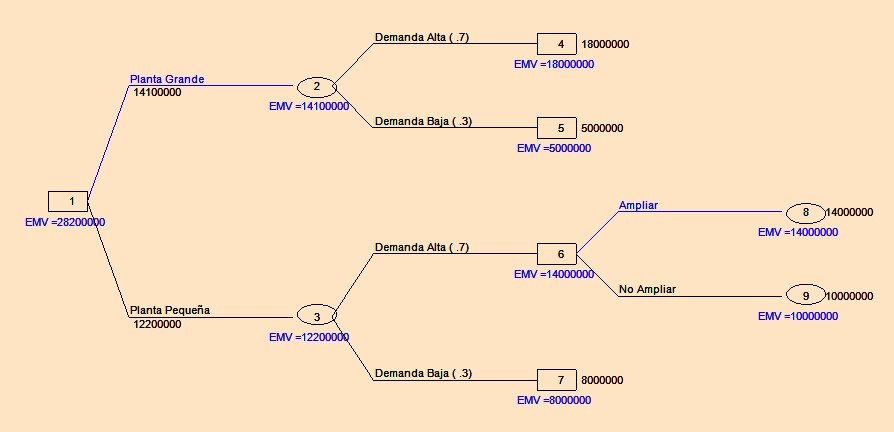
\includegraphics[width=1.0\linewidth,height=0.3\textheight]{arbol1.jpg}\\

\hspace{10mm}b)¿Qué debe hacer la gerencia para obtener el beneficio esperado más alto?\\

\justify
\normalsize De acuerdo al árbol y los datos observados se puede saber que conviene mejor la construcción de la planta grande desde el inicio.
\begin{center}
\section{El ejercicio planteado en el archivo (Nuevo):}
\end{center}

\justify
Un atribulado alumno debe decidir si estudiar o no para un examen. Si estudia, sacrificara un tiempo equivalente a 1.9 ptos. (Tiempo que puede dedicar a otros ramos). Conociendo sus capacidades, y dada su experiencia sabe que si estudia y el control está fácil se va a sacar un 6.5, pero si estudia y el control tiene una dificultad mediano o difícil se sacaría un 5.0 o un 2.0 respectivamente. Por otra parte, si no estudia y el control está fácil, mediano o difícil se sacaría un 4.5, 2.5, y un 1.5 respectivamente.
De acuerdo a la historia del curso hay un 30\% de probabilidades que el control esté fácil, un 50\% que esté mediano y un 20\% que esté difícil.
Por otro lado, se sabe que el profesor acostumbra a dar cierta información sobre la dificultad del control, la clase antes de éste. Sin embargo, esta información no es perfecta y su confiabilidad se puede describir por la siguiente tabla: \\
\begin{center}
\begin{tabular}{ | c | c | c | c | }
 \hline
 & Facil & Mediano & Dificil \\ \hline
Dice Facil & 0.8 & 0.2 & 0.1 \\
Dice Mediano & 0.1 & 0.7 & 0.3 \\
Dice Dificil & 0.1 & 0.1 & 0.6 \\ \hline
\end{tabular}
\end{center}

\hspace{10mm} a) Proponga y resuelva el árbol de decisión que se plantea al estudiante.\\

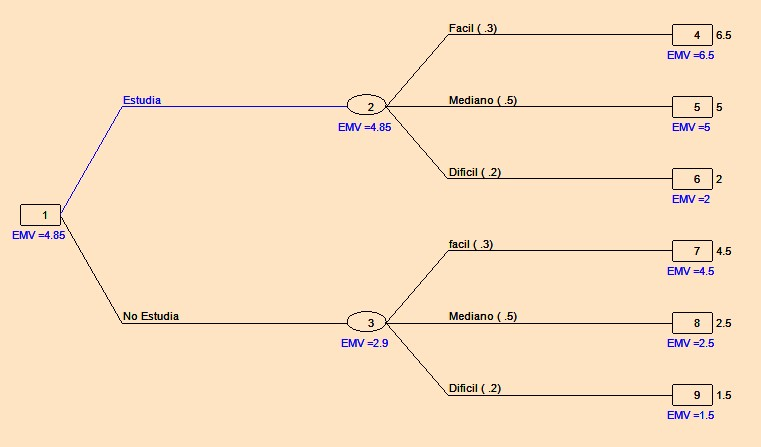
\includegraphics[width=1.0\linewidth,height=0.3\textheight]{arbol2.jpg}\\

\justify
Con la información que plantea del estudiante se puede observar una gran diferencia sobre la dedición de estudiar \emph{(4.85)} y si no estudia \emph{(2.9)}. Por lo cual la opción más adecuada es estudiar para el examen.\\

\hspace{10mm} b)Calcule el valor esperado de la información perfecta.\\

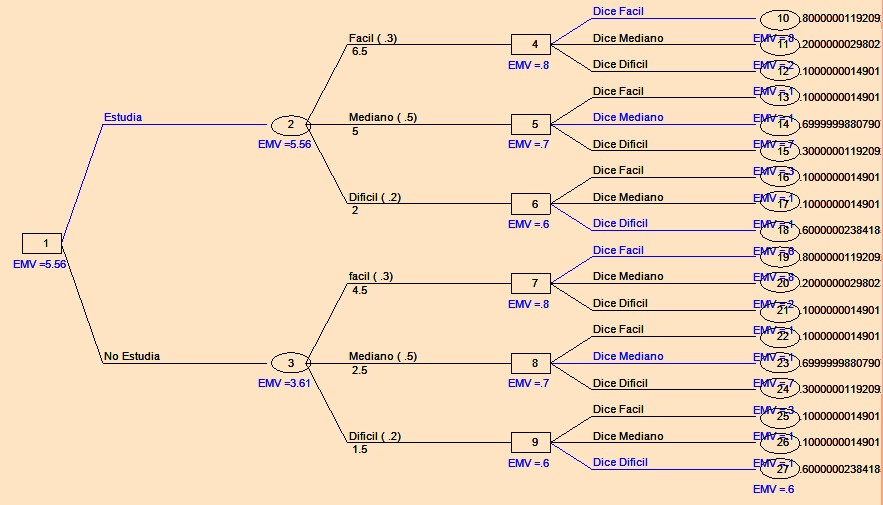
\includegraphics[width=1.0\linewidth,height=0.3\textheight]{arbol3.jpg}\\

\justify
De igual forma utilizando la información perfecta también podemos observar la gran diferencia sobre la dedición de estudiar \emph{(5.56)} y si no estudia \emph{(3.61)}. Por lo cual la opción más adecuada es estudiar para el examen.

\end{center}
\end{document}